\documentclass{article}%
\usepackage[T1]{fontenc}%
\usepackage[utf8]{inputenc}%
\usepackage{lmodern}%
\usepackage{textcomp}%
\usepackage{lastpage}%
\usepackage[head=40pt,margin=0.5in,bottom=0.6in]{geometry}%
\usepackage{graphicx}%
%
\title{\textbf{Trabajadores de la UCV protestaron por incumplimiento de contrato colectivo}}%
\author{El Nacional Web}%
\date{08/10/2018}%
%
\begin{document}%
\normalsize%
\maketitle%
\textbf{URL: }%
http://www.el{-}nacional.com/noticias/protestas/trabajadores{-}ucv{-}protestaron{-}por{-}incumplimiento{-}contrato{-}colectivo\_254835\newline%
%
\textbf{Periodico: }%
EN, %
ID: %
254835, %
Seccion: %
Protestas\newline%
%
\textbf{Palabras Claves: }%
UCV, Protestas, Denuncia\newline%
%
\textbf{Derecho: }%
2.3%
, Otros Derechos: %
NO\_TIENE%
, Sub Derechos: %
2.3.4%
\newline%
%
\textbf{EP: }%
SI\newline%
\newline%
%
\textbf{\textit{Representantes del sindicato de trabajadores de la institución manifestó en las instalaciones de la casa de estudios para exigir el respeto a las escalas salariales}}%
\newline%
\newline%
%
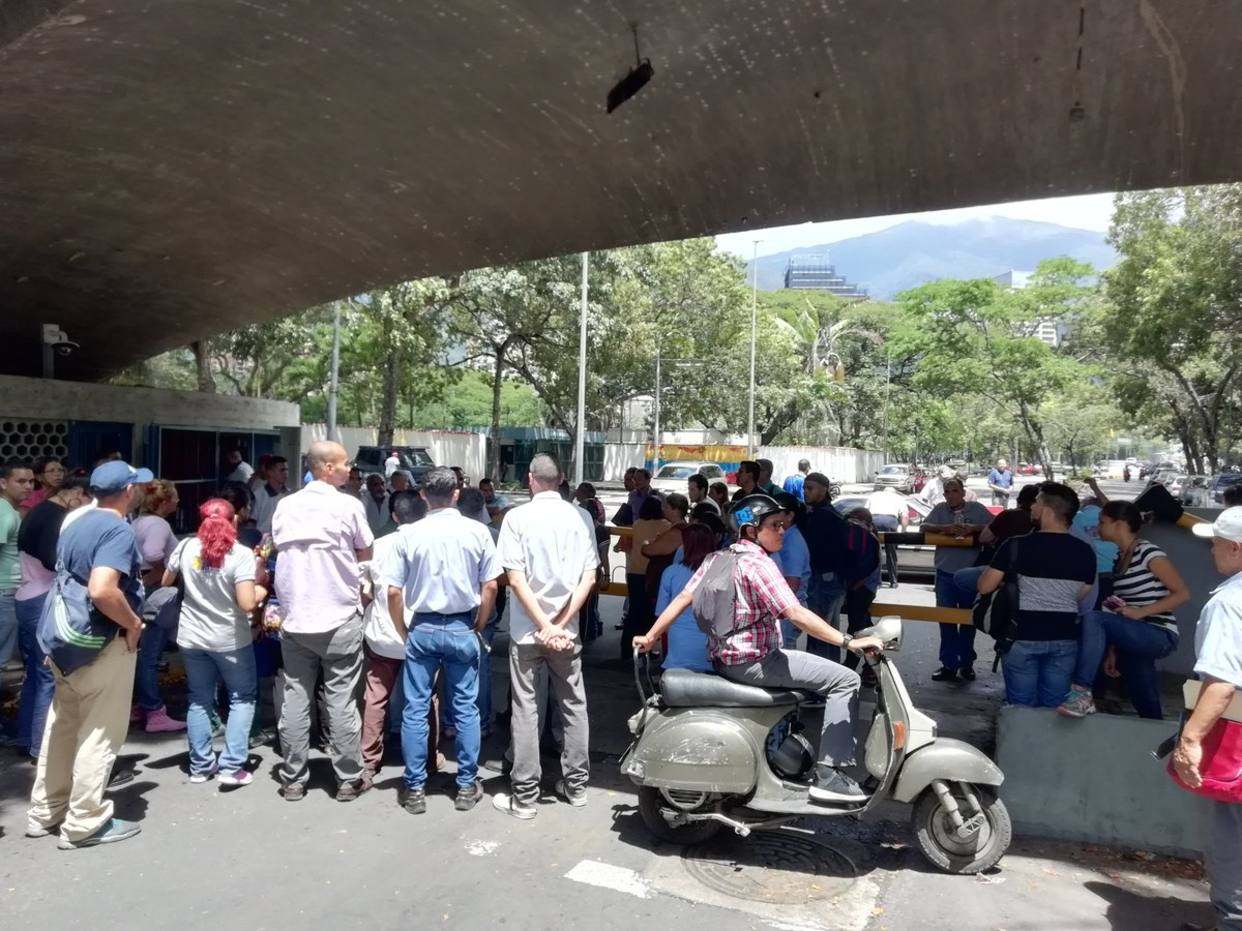
\includegraphics[width=300px]{3.jpg}%
\newline%
%
El sindicato de trabajadores de la Universidad Central de Venezuela protestaron este lunes en las instalaciones de la casa de estudios por el incumplimiento de los contratos colectivo y el respeto de las escala salariales.%
\newline%
%
Eduardo Sánchez, Presidente del~Sindicato de trabajadores de la UCV,~denunció~que el Jardín Botánico no cuenta con electricidad desde hace más de ocho~meses.%
\newline%
%
Además, Sanchéz anunció que este miércoles los trabajadores de la casa de estudios irán al Mnisterio de Educación Universitaria para exigir mejoras salariales.%
\newline%
%
Los empleados trancaron el paso vehícular desde tempranas horas de la mañana, sin embargo, el paso fue restablecido a las 12:00~pm.%
\newline%
%
\end{document}